%!TEX root = Projeto.tex
\subsection{Fluxos da informação no navegador}

\subsubsection{O navegador e seus subsistemas componentes}
A capacidade que software navegador tem para buscar informação, apresentá-la ao usuário e torná-la interativa é produto da cooperação de subsistemas responsáveis pela comunicação através da rede, a interpretação de código HTML, a representação visual das páginas, o gerenciamento de \poe{caches} e a execução de \scripts{}. Os navegadores divergem na forma de implementação desses subsistemas, mas em geral empregam arquiteturas que enfatizam aspectos não-funcionais como tolerância a falhas, utilização reduzida de recursos e segurança do ambiente de execução. Navegadores como Chrome, Internet Explorer e Safari utilizam separação de processos por aba de navegação \cite{Bright2016} para elevar o nível de isolamento entre as sessões de usuário; Firefox segue essa tendência ao adotar uma arquitetura de múltiplos processos em seus \poe{releases} mais recentes \cite{Nguyen2017}, coordenando até quatro processos de navegação compartilhados entre todas as abas. No âmbito da segurança da informação, a capacidade de execução em múltiplos processos faz com que o navegador isole, em contextos de alta restrição de permissões \poe{(sandboxes)}, quaisquer aplicações web anômalas que tentassem, por meio de \poe{crashes} deliberados, causar instabilidade do navegador ou do sistema operacional pela execução de código em contexto privilegiado \cite{Chromium2018_MPA}.

Em linhas gerais, \citeauthor{HTML5Rocks2011} descreve a colaboração entre seis subsistemas que compõem um navegador moderno, ilustrados pelo diagrama \ref{Fig: diagrama03}, e descritos no quadro \ref{Box: browserComponents}.

\begin{quadro}[h]
	\begin{framed}{\small
	\begin{description}
		\item [Interface do usuário:] expor os elementos interativos de que o usuário dispõe para comandar o navegador, como a barra de endereços, os comandos de navegação (``voltar'', ``avançar'', ``recarregar'') e os comandos de menu do navegador, incluindo os menus de contexto, atalhos, acesso às configurações e às extensões. A janela de interface do usuário hospeda, ainda, o componente de superfície (\poe{canvas}) responsável pela exibição do conteúdo tornado visível (``renderizado'') pelo subsistema Mecanismo do navegador.
		
		\item [Mecanismo do navegador:] comandar o mecanismo de visualização sob a demanda das ações originadas pela interface do usuário e, em resposta a esses comandos, sinalizar mudanças de estado que serão refletidas pela interface de usuário. Exemplo disso é o ciclo de carregamento de páginas da web, que dispara o \poe{download} de recursos de rede, a renderização desses recursos e a atualização da interface de usuário à medida em que as etapas do carregamento se sucedem.
		
		\item [Mecanismo de visualização:] ``renderizar'', ou transformar em conteúdo audiovisual, o fluxo de dados transferidos pelo subsistema de acesso à rede. O fluxo de dados carrega informação textual codificada nas linguagens HTML e CSS, e também dados binários em formato de imagem, áudio e vídeo. O mecanismo de visualização pode dar suporte à renderização de dados em formatos não vinculados à HTML, como documentos PDF e arquivos XML.
		
		\item [Acesso à rede:] conectar-se aos provedores de informação indicados por meio de URLs (\poe{uniform resource locators}) e estabelecer fluxos de dados sob diferentes protocolos como HTTP, HTTPS, Web Sockets, WebRTC e FTP.
		
		\item [Persistência de dados:] prover funcionalidades para armazenamento de dados persistentes, incluindo \poe{caches}, \poe{cookies}, suporte ao sistema de arquivos e as APIs para bancos de dados de escala reduzida como \poe{localStorage} e IndexedDB.
		
		\item [Interpretador de Javascript:] compilar e executar código na linguagem Javascript. ``V8'', ``Chakra'' e ``SpiderMonkey'' são os nomes dos subsistemas de interpretação de Javascript empregados pelos navegadores Chrome, Microsoft Edge e Firefox, respectivamente. Os diversos interpretadores aderem às especificações estabelecidas pelo consórcio ECMA sob o padrão ``ECMAScript'', que define a sintaxe e os recursos que devem ser suportados pela linguagem.
	\end{description}}
	\end{framed}
	\caption[Responsabilidades dos subsistemas componentes do navegador]{Responsabilidades dos subsistemas componentes do navegador. Adaptado de \cite{HTML5Rocks2011}}
	\label{Box: browserComponents}
\end{quadro}


%As responsabilidades desses subsistemas são segregadas entre processos distintos, o que eleva a capacidade do navegador de se manter funcional mesmo quando uma determinada página provoca uma falha de execução que termina seu processo hospedeiro \dubious{(e falta ilustrar essa segregação)}

\begin{figure}[h]
	\centering
	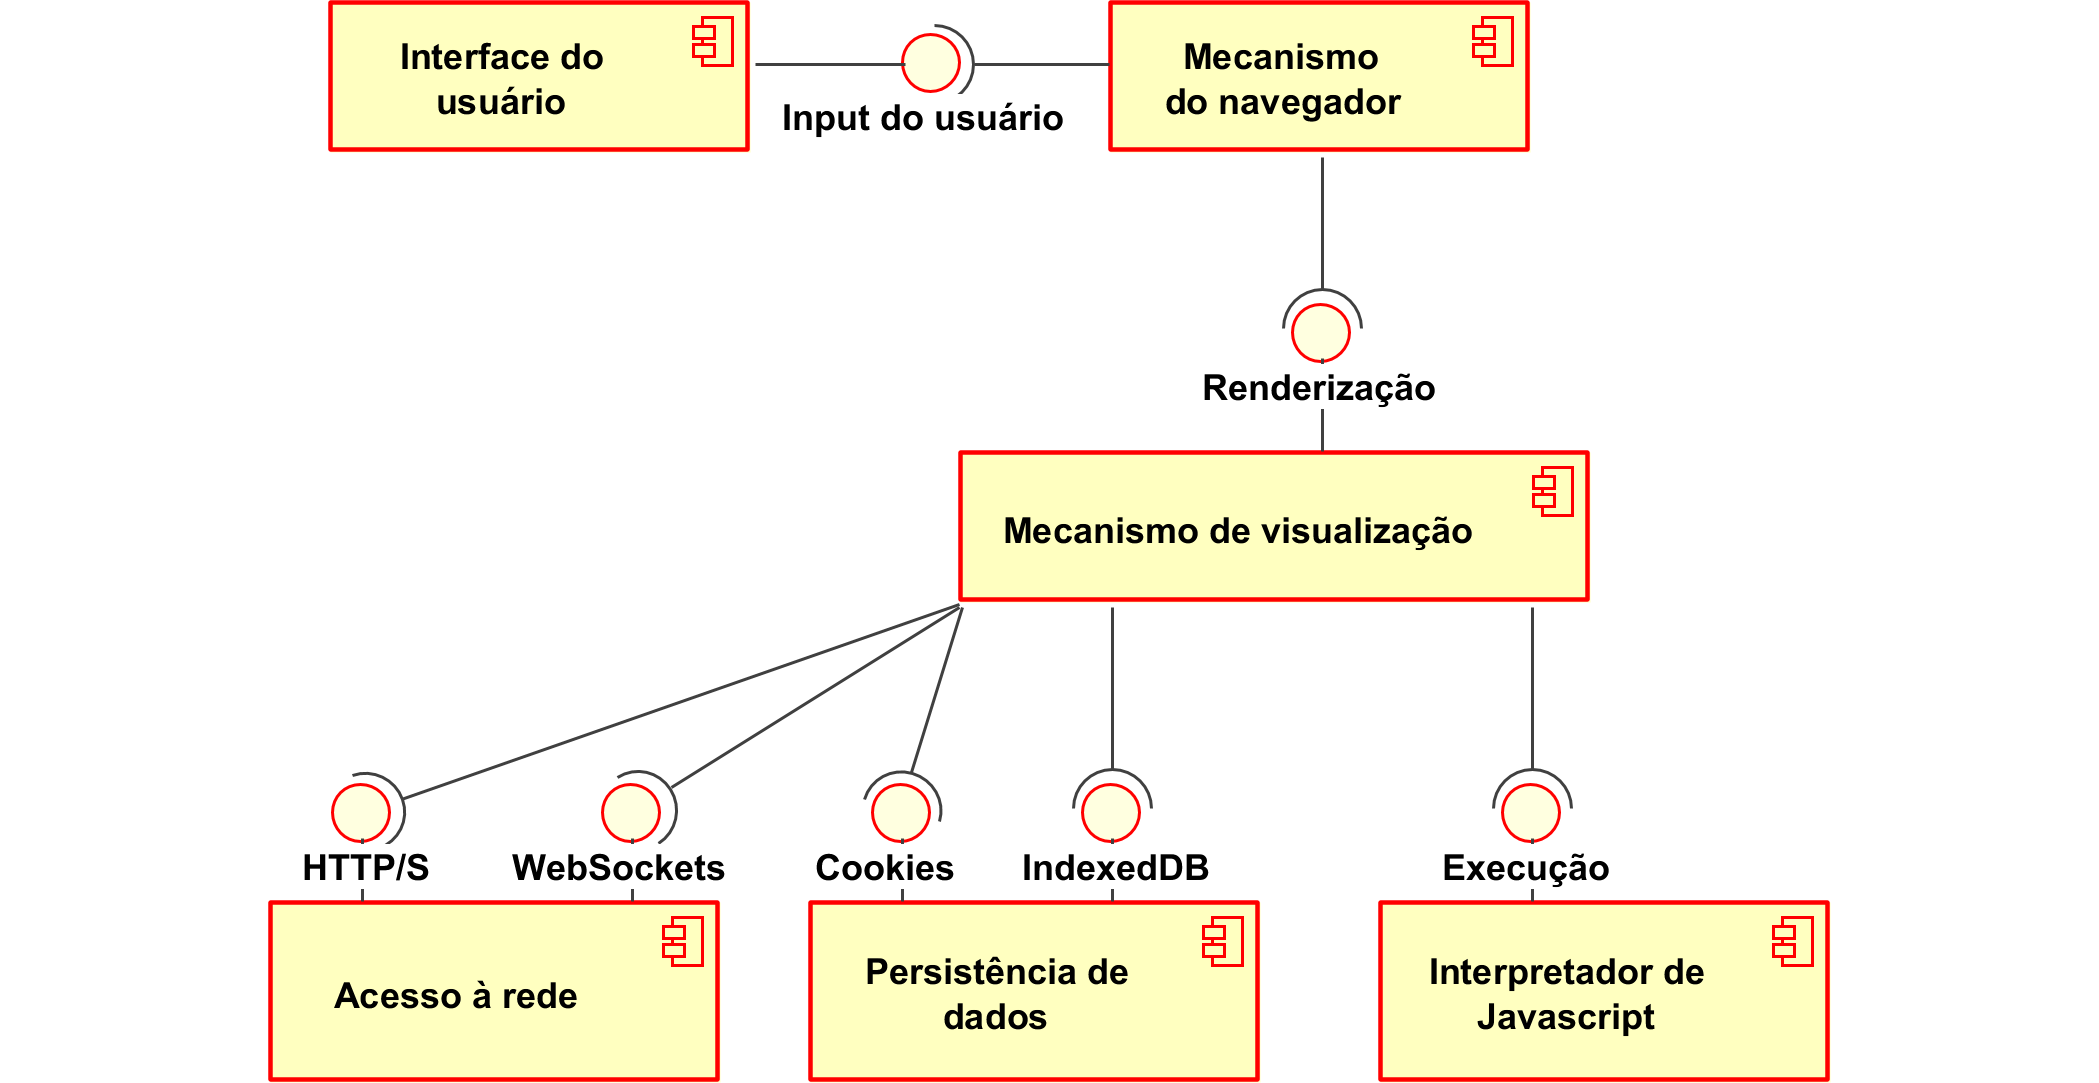
\includegraphics[width=12cm]{diagramas/componentes-navegador.png}
	\label{Fig: diagrama03}
	\caption[Componentes do navegador de código aberto Chromium]{Componentes do navegador de código aberto Chromium. Adaptado de \cite{Chromium2018_MPA, Chromium2018_MPRL, HTML5Rocks2011}}
\end{figure}

% VELHARIAS SEM SUBSTÂNCIA....
% Sob o ponto de vista da segurança da informação, cabem algumas observações:

% \begin{alineas}
% 	\item Os subsistemas do navegador podem apresentar conjuntos próprios de vulnerabilidades, inerentes ao funcionamento e à implementação de cada um;
% 	\item O inter-relacionamento entre esses subsistemas estabelece fluxos de informação que, por sua vez, também podem apresentar vulnerabilidades;
% 	\item Ao longo do tempo, a descoberta de vulnerabilidades e a evolução dos navegadores contribuíram para o estabelecimento de políticas para a segurança na web;
% 	\item A manutenção de certas funcionalidades, necessárias para o funcionamento das aplicações web modernas, comprometeu a capacidade do navegador de se manter imune a todas as vulnerabilidades de vazamento de informação possíveis.
% \end{alineas}

% \subsubsection{Ciclo de vida de uma página da web}

% O ciclo de vida de uma página da web é a sequência de atividades executadas pelo navegador durante os processos de carga, exibição e interação do usuário com o conteúdo visualizado, perdurando até a ação de descarregamento da página, desencadeada pela navegação do usuário ou pelo fechamento da janela do navegador. A informação criada e mantida dentro do ciclo de vida de uma página é volátil, sendo descartada no descarregamento. Para que se torne persistente, a informação precisa ser transmitida em uma requisição HTTP ou armazenada localmente em estruturas como \poe{cookies}, \poe{localStorage} ou IndexedDB, sempre a critério do desenvolvedor da aplicação web de que a página fizer parte.

% É durante o ciclo de vida da página que ocorrem os eventos que levam às vulnerabilidades relevantes para este trabalho. Não apenas a informação requisitada pelo navegador no momento da carga da página, mas também toda informação produzida pela interação do usuário com os elementos de página, compõem o conjunto dados vulneráveis a vazamento. Por meio de disparo de eventos do DOM, um {\script} pode capturar a sequência de ações desempenhadas pelo usuário enquanto este aciona os controles de \poe{mouse}, digita caracteres pelo teclado e efetua rolagem de tela. Mesmo eventos emitidos por ações que não dependam de interação do usuário, como mudanças de estado do DOM e o carregamento de recursos oriundos da rede, podem ser capturados e preservados em uma linha do tempo de acontecimentos que revela toda a experiência do usuário durante o ciclo de vida de uma página.

\subsubsection{Fluxos de informação violadores da privacidade do usuário}

O estudo empírico de \citeauthor{Jang2010}, conduzido em \citeyear{Jang2010} tendo como alvo os 50.000 sites mais visitados do mundo\footnote{O serviço Alexa provê serviços de análise da visitação de sites, sob consulta. \url{https://www.alexa.com/topsites}}, evidenciou uma variedade de fluxos capazes de comprometer a privacidade dos dados de usuário em nos sites \poe{sites} de grande circulação. Os autores descrevem quatro efeitos desses fluxos: roubo de \poe{cookies}, sequestro do endereço corrente (\poe{location hijacking}), espionagem de histórico (\poe{history sniffing}), e observação do comportamento do usuário. Isoladamente ou em conjunto, os fluxos violadores da privacidade podem ser acionados a partir de um único \script{} comprometido, sem que o desenvolvedor do \poe{site} afetado tenha conhecimento ou o poder de neutralizá-los preventivamente.

\begin{alineas}
	\item Roubo de \poe{cookies}. Como qualquer \script{} incorporado, código malicioso tem acesso à toda informação contida na página hospedeira, incluindo informação armazenada em \poe{cookies}, e permissão para enviar essa informação para outros agentes pelo uso de alguma das diversas maneiras de se invocar recursos remotos enumeradas na seção \ref{Secao: Vulnerabilidades_MecanismosPropagacao}. \poe{Cookies} expostos dessa maneira podem ser utilizados para forjar requisições posteriores em nome do usuário, agravando o potencial de comprometimento de informação.
	\item Sequestro do endereço corrente. O endereço URL corrente do navegador é um valor exposto pelo DOM na propriedade |document.location|. Todo código Javascript tem poder de ler e modificar essa propriedade, cuja alteração causa uma imediata carga do endereço especificado. Um \script{} pode aproveitar-se desse comportamento para redirecionar informação contida na página.
	\item Espionagem de histórico. Embora o histórico de navegação propriamente dito, correspondente à sequência de URLs visitadas, não seja exposto pelo DOM, uma forma de ataque conhecida como XSHM \poe{(Cross Site History Manipulation)} \cite{OWASP:XSHM} revela informação suficiente para que seja possível deduzir, por exemplo, se o usuário fez \poe{login} em determinada aplicação-alvo. Um \script{} pode valer-se dessa dedução para emitir requisições mal-intencionadas para esse alvo em nome do usuário corrente.
	\item Observação do comportamento do usuário. \Scripts{} têm a capacidade de registrar código ``ouvinte'' de eventos derivados da interação do usuário com a página web, como movimentos de \poe{mouse}, cliques, acionamento de teclado e rolagem de tela. Essa informação pode ser retransmitida para outros agentes na internet, que poderão acompanhar as ações do usuário em tempo real.
\end{alineas}

\citeauthor{Jang2010} afirmam que as causas que viabilizam a existência desses fluxos são a natureza dinâmica da linguagem Javascript, sua falta de mecanismos de isolamento entre \scripts{}, e a granularidade incoerente das políticas como a SOP.

% \begin{todo}
% Pontos a considerar:

% \begin{alineas}
% 	\item O navegador da web é um cliente da internet.
% 	\item O ciclo de vida de uma página é "curto" (cada página, uma aplicação diferente? um contexto de execução diferente?)
% 	\item Onde está a informação no navegador, e qual sua duração possível?
% 	\begin{alineas}
% 		\item Endereço (URL) corrente
% 		\item Requisição (pode ser da página como de "sub-recursos" como imagens, iframes, scripts, estilos, xhr...)
% 		\item Resposta
% 		\item Estrutura da página (DOM)
% 		\item Eventos do navegador/DOM
% 		\item Closures
% 		\item Pilha de chamadas
% 		\item Extensões do navegador
% 		\item Caches
% 		\item Cookies
% 		\item Local DB
% 		\item Em HTTPS, temos mais fluxos?
% 	\end{alineas}
% \end{alineas}

% Então será possível indicar quais dos fluxos estão protegidos contra vazamento de informação, e como estão. E consequentemente quais fluxos não estão cobertos.
% \end{todo}
